\documentclass[12pt]{article}
\usepackage[utf8]{inputenc}
\usepackage[T1]{fontenc}
\usepackage[polish]{babel}
\usepackage{geometry}
\usepackage{tabularx}
\usepackage[table,xcdraw,dvipsnames]{xcolor}
\usepackage{tabularx}
\usepackage{color}
\usepackage{subfig}
\usepackage{sidecap}
\usepackage{wrapfig}
\usepackage{float}
\usepackage{enumerate}
\usepackage{graphicx}
\usepackage{multirow}
\usepackage{hyperref}
\usepackage{titlesec}
\usepackage{amsmath}
\usepackage{anyfontsize}
\usepackage{indentfirst}
\usepackage{listings}
\usepackage{multicol}
\usepackage{pgfplots}
\usepackage{fancyhdr}

\newgeometry{tmargin=1.8cm,bmargin=1.8cm,lmargin =1.8cm,rmargin=1.8cm}
\begin{document}

\newcommand{\zdjecie}[3]
{
    \begin{figure}[H]
        \renewcommand{\figurename}{Rys.}
        \centering
        \includegraphics[width=\textwidth]{#1}
        \caption{#2}
        \label{#3}
    \end{figure}
}

\begin{table}[H]
    \centering
    \renewcommand{\arraystretch}{1.5}
    \begin{tabularx}{\textwidth}{|X|X|}
    \hline
    \multicolumn{2}{|c|}{\large\textbf{Notatka służbowa nr 3}} \\ \hline
    Temat:          & Automatyzacja modelu linii produkcyjnej (Magazyn)    \\ \hline
    Wykonanie:      & Zuzanna Mejer, 259382   \\ \hline
    Termin zajęć:   & poniedziałek TP, 10:55  \\ \hline  
    Data:           & 28.11.2022    \\ \hline
    \end{tabularx}
    \end{table}

\section{Cel ćwiczenia}
Celem ćwiczenia było zapoznanie się z modelem linii produkcyjnej oraz napisanie programu obsługującego jego część (na stanowisku pierwszym - Magazyn). Do wykonania zadania wykorzystano sterownik TSX Micro 3721 firmy Schneider Automation z oprogramowaniem w wersji V1.6 oraz program PL7PRO.

\section{Uruchomienie oprogramowania i konfiguracja sterownika}
Przed rozpoczęciem pracy ze sterownikiem, należało uruchomić i skonfigurować oprogramowanie
i sterownik. W tym celu wykonano poniższe czynności.
\begin{enumerate}
    \item Uruchomiono program PL7PRO i utworzono nowy projekt. Pojawiło się okno, w którym należało wybrać odpowiedni sterownik (TSX Micro), model wraz z wersją oprogramowania (TSX
    3721 V1.5 - ze względu na brak wersji V1.6) oraz zaznaczyć ,,No'' przy Grafcet (rys. \ref{konfiguracja1}).
    \begin{figure}[H]
        \centering
        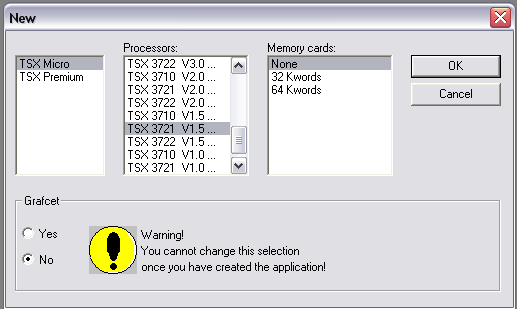
\includegraphics[scale=0.8]{./zdjecia/konfiguracja.png}
        \caption{Uruchomienie programu PL7PRO}
        \label{konfiguracja1}
    \end{figure}
    \item Następnie zdefiniowano typy modułów sterownika. Wybrano opcję \textit{Configuration $ \rightarrow $ Hardware configuration} i wpisano odpowiednie typy modułów (rys.\ref{hardware_conf}). W przypadku stanowiska pierwszego były one następujące: 
    \begin{itemize}
        \item moduł wejść i wyjść cyfrowych - TSX DMZ 28DR
        \item moduł wejść analogowych - TSX AEZ 414
        \item moduł wyjść analogowych - TSX ASZ 200
    \end{itemize}
    \begin{figure}[H]
        \centering
        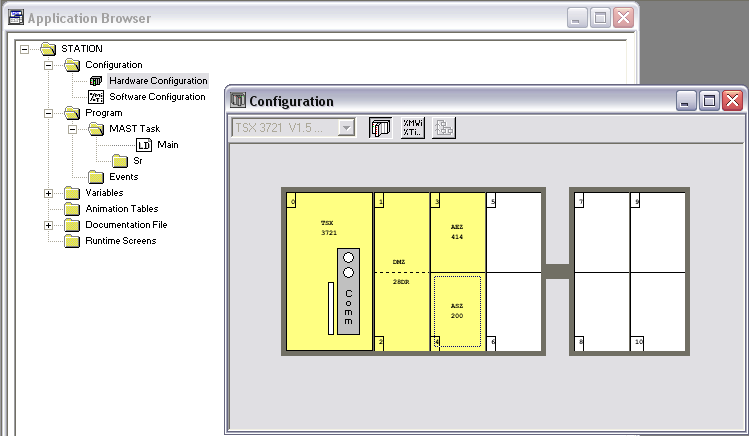
\includegraphics[scale=0.6]{./zdjecia/hardware_conf.png}
        \caption{Konfiguracja hardware'u - określanie modułów sterownika}
        \label{hardware_conf}
    \end{figure}
    \item Wybrano język programowania drabinkowy we właściwościach programu głównego (rys.\ref{LD}).
    \begin{figure}[H]
        \centering
        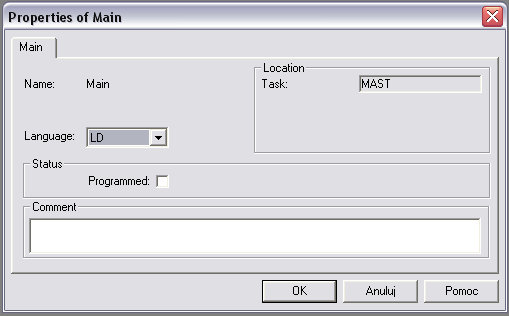
\includegraphics[scale=0.8]{./zdjecia/main_LD.png}
        \caption{Wybranie języka LD}
        \label{LD}
    \end{figure}
\end{enumerate}


\section{Moduł Magazyn}
\subsection{Zasady działania}
Moduł MAGAZYN składa się z zasobnika z elementami do obróbki, popychacza transportującego element do punktu, z którego jest pobierany za pomocą ramienia z przyssawką i podawany na następny moduł. 

\subsection{Program obsługi w języku drabinkowym}
Program składa się łącznie z 6 szczebli. Pierwszy szczebel resetuje wszystkie ustawienia do ustawień początkowych (cofnięty popychacz, wyłączone ssanie, ramię przesunięte w kierunku kolejnego stanowiska). Został on stworzony na wypadek pojawienia się jakiegoś błędu podczas któregokolwiek etapu działania tej części linii produkcyjnej. Opcja ta przydała się, na przykład, gdy podany do zasobnika został klocek z dziurami, do którego przyssawka nie mogła się przyczepić, co zastopowało działanie całej linii. Po wciśnięciu przycisku $\%I1.10$ na pulpicie, wszystkie elementy powróciły do stanu początkowego, a nadzorujący mógł wyciągnąć wadliwy klocek.

\zdjecie{./zdjecia/1galaz.png}{Pierwsza gałąź programu - RESET}{1galaz}

Najpierw wykonywane jest resetowanie: $\%Q2.0$ - wysunięcia popychacza, $\%Q2.1$ - przesunięcia ramienia w kierunku popychacza oraz $\%Q2.4$ - włączenia ssania. Następnie wykonywane jest: $\%Q2.2$ - przesunięcie ramienia w kierunku stanowiska pomiarowego oraz $\%Q2.3$ - wyłączenie ssania.

Od drugiego szczebla zaczyna się już właściwy program. Element znajdujący się w komorze popychacza (negacja $\%I1.6$) uruchamia timer On-Delay, który odlicza 5 sekund. Po tym czasie uruchamiane jest wysunięcie popychacza ($\%Q2.0$). Po kolejnych 5 sekundach od wypchnięcia elementu przez popychacz, jest on cofany.

\zdjecie{./zdjecia/2galaz.png}{Druga gałąź programu - wysunięcie popychacza}{2galaz}

Jeżeli popychacz został wysunięty ($\%I1.1$), uruchamiane zostaje przesunięcie ramienia w kierunku popychacza ($\%Q2.1$). Zanim jednak to nastąpi, należy zresetować przesunięcie ramienia w kierunku stanowiska pomiarowego ($\%Q2.2$).

\zdjecie{./zdjecia/3galaz.png}{Trzecia gałąź programu - przesunięcie ramienia w kierunku popychacza}{3galaz}

Kiedy ramię podajnika jest w pozycji maksymalnie wychylonej w kierunku magazynu ($\%I1.2$), następuje włączenie ssania ($\%Q2.4$). Zanim jednak to nastąpi, należy pamiętać o zresetowaniu wyłączenia ssania ($\%Q2.3$).

\zdjecie{./zdjecia/4galaz.png}{Czwarta gałąź programu - włączenie ssania}{4galaz}

Kiedy element jest przyssany do przyssawki ramienia ($\%I1.5$), następuje najpierw reset przesunięcia ramienia w kierunku popychacza ($\%Q2.1$) i następnie przesunięcie ramienia w kierunku stanowiska pomiarowego ($\%Q2.2$).

\zdjecie{./zdjecia/5galaz.png}{Piąta gałąź programu - przesunięcie ramienia w kierunku stanowiska pomiarowego}{5galaz}

Ostatnim etapem jest wyłączenie ssania ($\%Q2.3$) po tym, gdy ramię podajnika znajdzie się w pozycji maksymalnie wychylonej w kierunku stanowiska pomiarowego ($\%I1.3$). Zanim to nastąpi, musi zostać zresetowane włączenie ssania ($\%Q2.4$).

\zdjecie{./zdjecia/6galaz.png}{Szósta gałąź programu - wyłączenie ssania}{6galaz}

\subsection{Działanie}
Po wykryciu elementu w zasobniku, popychacz czeka 5 sekund, a następnie wysuwa się, popychając element w wyznaczone miejsce. Po kolejnych 5 sekundach, popychacz cofa się. W tym czasie ramię podajnika przesuwa się w kierunku magazynu. Następnie włączane jest ssanie i przyssawka przyczepia się do elementu. Wtedy ramię przesuwa się w kierunku stanowiska pomiarowego. Wyłączane jest ssanie, element został przeniesiony w wyznaczone miejsce i tym samym kończy się cykl. Program działa także poprawnie, gdy w zasobniku znajduje się więcej niż jeden element. Dodatkowa opcja resetu jest przydatna na wypadek wystąpienia niespodziewanych przeszkód.

\section{Podsumowanie}
Program działał zgodnie z założeniami. Pisanie programu oraz testowanie nie sprawiło większych problemów. Ćwiczenie pozwoliło wykorzystać poznaną wiedzę w praktyce w ciekawy sposób. Ponadto, umożliwiło utrwalenie konfiguracji i obsługi sterownika TSX Micro oraz programu PL7PRO.



\end{document}